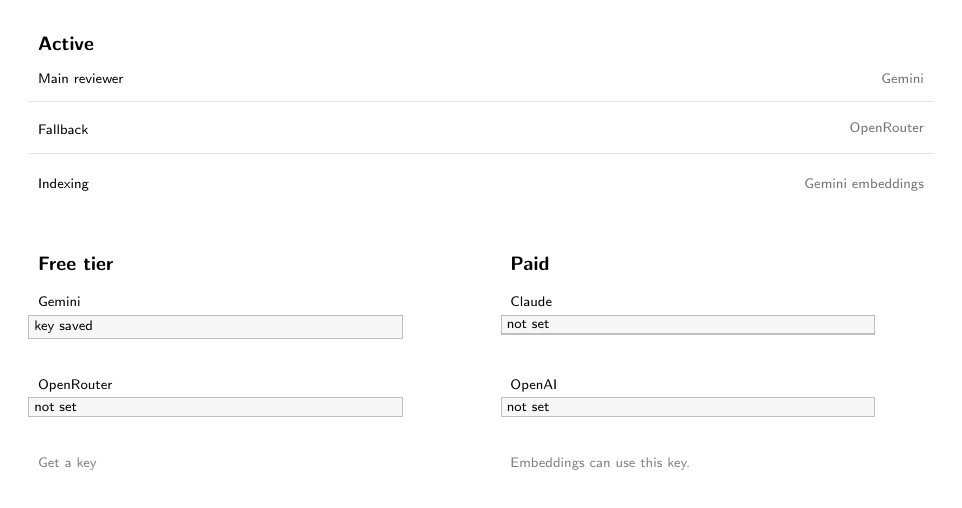
\begin{tikzpicture}[x=1cm,y=1cm]
  \wfchrome{AI providers}{6.05}

  \wfpanel{3.40}{5.15}{11.85}{2.55}
  \node[anchor=north west, font=\sffamily\bfseries\scriptsize] at (3.55,7.50) {Active};
  \node[anchor=west, font=\sffamily\tiny] at (3.55,6.85) {Main reviewer};
  \node[anchor=east, font=\sffamily\tiny, text=black!55] at (15.05,6.85) {Gemini};
  \draw[black!10] (3.55,6.55) -- (15.05,6.55);
  \node[anchor=west, font=\sffamily\tiny] at (3.55,6.20) {Fallback};
  \node[anchor=east, font=\sffamily\tiny, text=black!55] at (15.05,6.20) {OpenRouter};
  \draw[black!10] (3.55,5.90) -- (15.05,5.90);
  \node[anchor=west, font=\sffamily\tiny] at (3.55,5.50) {Indexing};
  \node[anchor=east, font=\sffamily\tiny, text=black!55] at (15.05,5.50) {Gemini embeddings};

  \wfpanel{3.40}{0.35}{5.75}{4.55}
  \node[anchor=north west, font=\sffamily\bfseries\scriptsize] at (3.55,4.70) {Free tier};
  \node[anchor=north west, font=\sffamily\tiny] at (3.55,4.20) {Gemini};
  \node[anchor=north west, draw=black!25, fill=black!3, font=\sffamily\tiny, inner sep=2pt, text width=4.6cm] at (3.55,3.85) {key saved};
  \node[anchor=north west, font=\sffamily\tiny] at (3.55,3.15) {OpenRouter};
  \node[anchor=north west, draw=black!25, fill=black!3, font=\sffamily\tiny, inner sep=2pt, text width=4.6cm] at (3.55,2.80) {not set};
  \node[anchor=north west, font=\sffamily\tiny, text=black!50] at (3.55,2.15) {Get a key};

  \wfpanel{9.40}{0.35}{5.85}{4.55}
  \node[anchor=north west, font=\sffamily\bfseries\scriptsize] at (9.55,4.70) {Paid};
  \node[anchor=north west, font=\sffamily\tiny] at (9.55,4.20) {Claude};
  \node[anchor=north west, draw=black!25, fill=black!3, font=\sffamily\tiny, inner sep=2pt, text width=4.6cm] at (9.55,3.85) {not set};
  \node[anchor=north west, font=\sffamily\tiny] at (9.55,3.15) {OpenAI};
  \node[anchor=north west, draw=black!25, fill=black!3, font=\sffamily\tiny, inner sep=2pt, text width=4.6cm] at (9.55,2.80) {not set};
  \node[anchor=north west, font=\sffamily\tiny, text=black!50] at (9.55,2.15) {Embeddings can use this key.};
\end{tikzpicture}
